% Cây policy theo source đã khóa; không biểu diễn tần suất chuyển hành động.
\documentclass[10pt]{article}
\usepackage[T1]{fontenc}
\usepackage{lmodern}
\usepackage[paperwidth=180mm,paperheight=183mm,margin=4mm]{geometry}
\usepackage{tikz}
\usetikzlibrary{arrows.meta}
\pagestyle{empty}
\setlength{\parindent}{0pt}
\definecolor{ink}{HTML}{1F3445}
\definecolor{teal}{HTML}{126B80}
\begin{document}
\centering
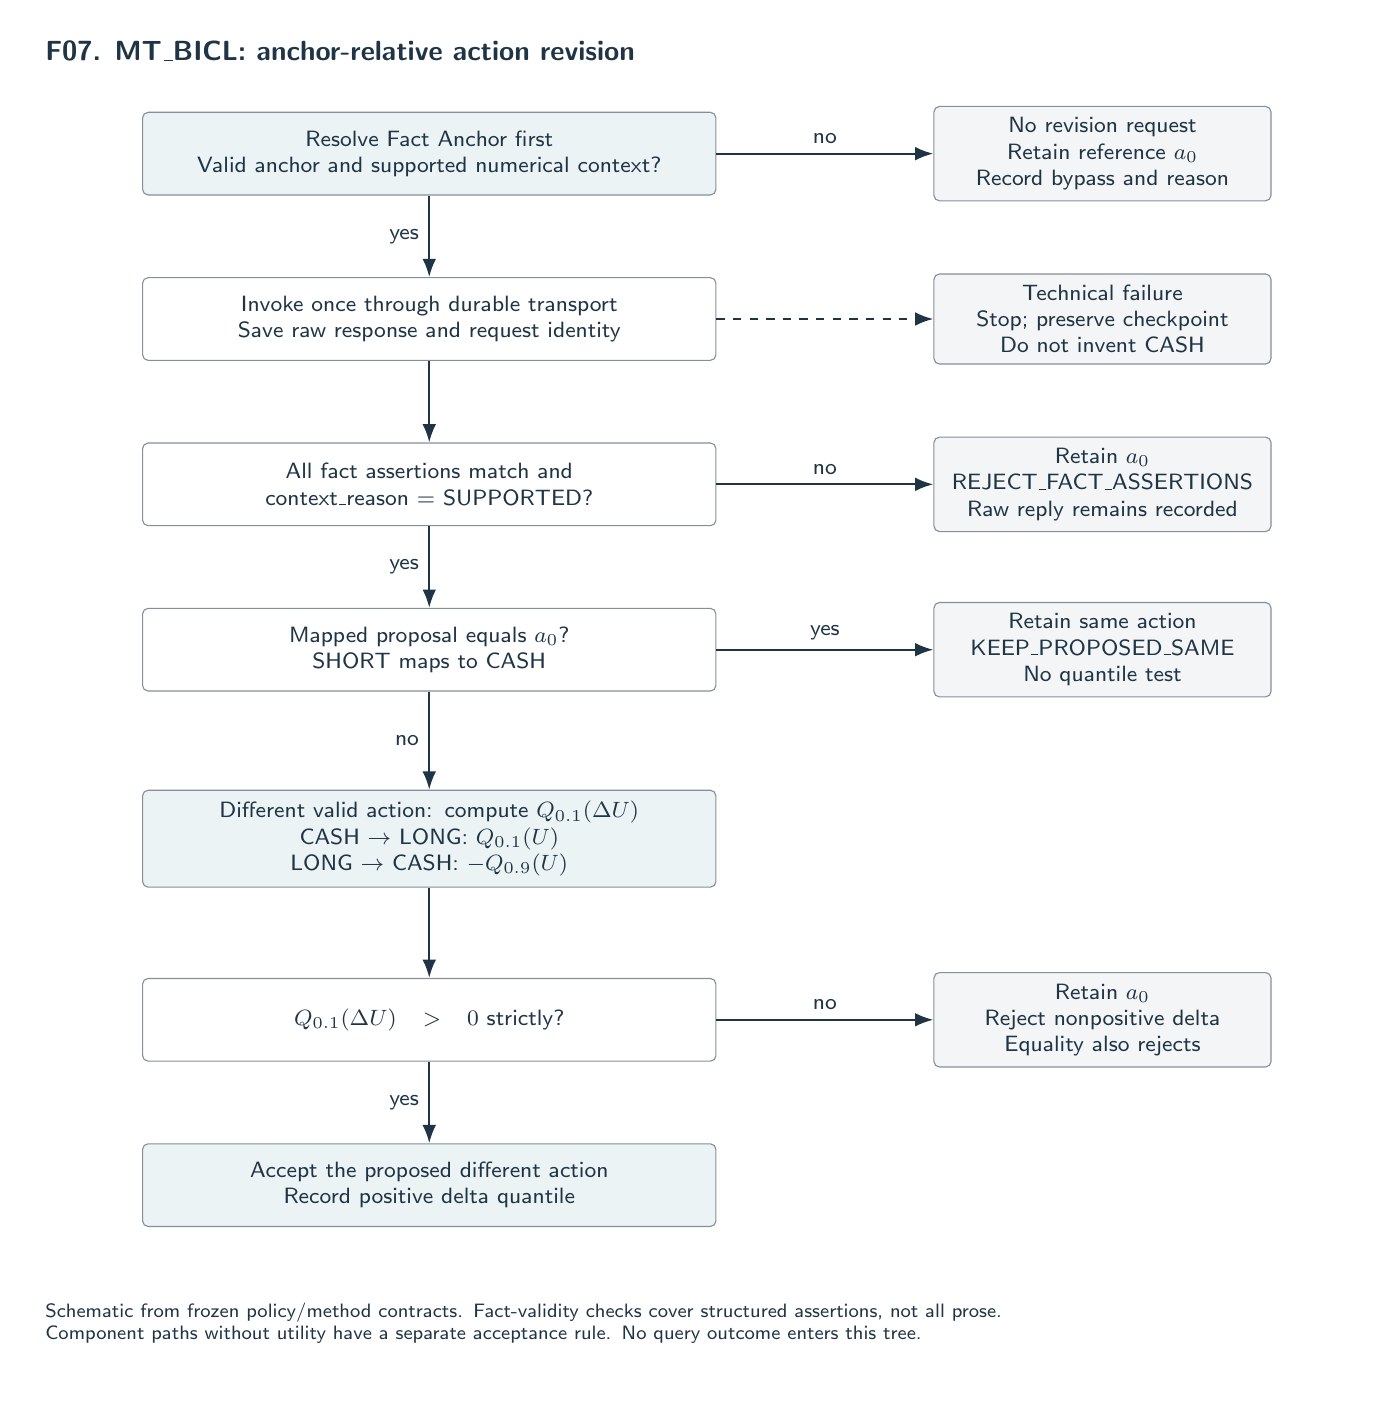
\begin{tikzpicture}[x=1cm,y=1cm,>=Latex,font=\sffamily\footnotesize,text=ink,
 box/.style={draw=ink!55,rounded corners=2pt,align=center,text width=7cm,minimum height=1.05cm,inner sep=4pt},
 side/.style={box,text width=4.0cm,fill=ink!5},flow/.style={->,thick,draw=ink}]
\path[use as bounding box] (0,0) rectangle (17,17.2);
\node[anchor=west,font=\sffamily\bfseries] at (.1,16.9) {F07. MT\_BICL: anchor-relative action revision};
\node[box,fill=teal!8] (start) at (5.1,15.6) {Resolve Fact Anchor first\\Valid anchor and supported numerical context?};
\node[side] (bypass) at (13.65,15.6) {No revision request\\Retain reference $a_0$\\Record bypass and reason};
\draw[flow] (start.east) -- node[above] {no} (bypass.west);
\node[box] (reply) at (5.1,13.5) {Invoke once through durable transport\\Save raw response and request identity};
\draw[flow] (start) -- node[left] {yes} (reply);
\node[side] (error) at (13.65,13.5) {Technical failure\\Stop; preserve checkpoint\\Do not invent CASH};
\draw[flow,dashed] (reply.east) -- (error.west);
\node[box] (facts) at (5.1,11.4) {All fact assertions match and\\context\_reason = SUPPORTED?};
\draw[flow] (reply) -- (facts);
\node[side] (invalid) at (13.65,11.4) {Retain $a_0$\\REJECT\_FACT\_ASSERTIONS\\Raw reply remains recorded};
\draw[flow] (facts.east) -- node[above] {no} (invalid.west);
\node[box] (same) at (5.1,9.3) {Mapped proposal equals $a_0$?\\SHORT maps to CASH};
\draw[flow] (facts) -- node[left] {yes} (same);
\node[side] (keep) at (13.65,9.3) {Retain same action\\KEEP\_PROPOSED\_SAME\\No quantile test};
\draw[flow] (same.east) -- node[above] {yes} (keep.west);
\node[box,fill=teal!8] (delta) at (5.1,6.9) {Different valid action: compute $Q_{0.1}(\Delta U)$\\CASH $\to$ LONG: $Q_{0.1}(U)$\\LONG $\to$ CASH: $-Q_{0.9}(U)$};
\draw[flow] (same) -- node[left] {no} (delta);
\node[box] (gate) at (5.1,4.6) {$Q_{0.1}(\Delta U)>0$ strictly?};
\draw[flow] (delta) -- (gate);
\node[side] (reject) at (13.65,4.6) {Retain $a_0$\\Reject nonpositive delta\\Equality also rejects};
\draw[flow] (gate.east) -- node[above] {no} (reject.west);
\node[box,fill=teal!8] (accept) at (5.1,2.5) {Accept the proposed different action\\Record positive delta quantile};
\draw[flow] (gate) -- node[left] {yes} (accept);
\node[anchor=west,align=left,text width=16.5cm,font=\sffamily\scriptsize] at (.1,.75)
 {Schematic from frozen policy/method contracts. Fact-validity checks cover structured assertions, not all prose.\\Component paths without utility have a separate acceptance rule. No query outcome enters this tree.};
\end{tikzpicture}
\end{document}
